\newpage
\section{Auswertung}

\subsection{a)}

    \noindent
    Bei den Messungen wurde der Photostrom gegen die Gegenspannung gemessen. 
    Aufgrund der $\sqrt{I} \propto  U$ Relation wird $\sqrt{I} $ gegen $  U$ aufgetragen.\\
    Durch diese Werte lässt sich dann eine Ausgleichgerade ziehen. Der Schnittpunkt dieser Gerade mit der x-Achse beschreibt dann die 
    Grenzspannung $U_{\symup{g}}$ bei der gerade keine Elektronen mehr die Anode erreichen. 
    Wenn die Ausgleichsgerade durch $y = a \cdot x +b$ beschrieben wird, dann berechnet sich die Grenzspannung mittels: 
    \noindent

    \begin{equation}
        U_{\symup{g}} = -  \frac{a}{b}.
    \end{equation}

    \begin{align}
        \text{gelb:  }   \quad     &a = (-\num{11.3}\pm \num{0.8})*10^{-5} \si{\ampere^{\frac{1}{2}}\per\volt} \nonumber\\
                        &b = (\num{1.06}\pm \num{0.34})*10^{-5} \si{\ampere} \nonumber\\
                        & \rightarrow U_{\symup{g}} = \SI{0.63 \pm 0.05}{\volt}
    \end{align}         

    \begin{align}
        \text{grün:  }   \quad     &a = (-\num{16.2}\pm \num{0.5})*10^{-5} \si{\ampere^{\frac{1}{2}}\per\volt} \nonumber\\
                            &b = (\num{8.75}\pm \num{0.19})*10^{-5} \si{\ampere} \nonumber\\
                            & \rightarrow U_{\symup{g}} = \SI{0.54 \pm 0.021}{\volt}
    \end{align}

    \begin{align}
        \text{violett:  }  \quad      &a = (-\num{11.63}\pm \num{0.2})*10^{-5} \si{\ampere^{\frac{1}{2}}\per\volt} \nonumber\\
                               &b = (\num{13.09}\pm \num{0.15})*10^{-5} \si{\ampere} \nonumber\\
                               & \rightarrow U_{\symup{g}} = \SI{1.126 \pm 0.023}{\volt}
    \end{align}

    \noindent
    Werden die Daten \ref{tab:gelb},\ref{tab:green},\ref{tab:violett} dann geplottet ergeben sich folgenede Plots:
    \noindent

    \begin{figure}[H]
        \centering
        \includegraphics[width=0.8\textwidth]{build/plots/sqrtgelb.pdf}
        \caption{Die Wurzel des Photostrom, gemessen für gelbes Licht, aufgetragen gegen die Spannung. Zusätzlich nch mit mit Ausgleichgerade.}
        \label{img:sqrtgelb}
    \end{figure}

    \begin{figure}[H]
        \centering
        \includegraphics[width=0.8\textwidth]{build/plots/sqrtgreen.pdf}
        \caption{Die Wurzel des Photostrom, gemessen für grünes Licht, aufgetragen gegen die Spannung. Zusätzlich nch mit mit Ausgleichgerade.}
        \label{img:sqrtgruen}
    \end{figure}

    \begin{figure}[H]
        \centering
        \includegraphics[width=0.8\textwidth]{build/plots/sqrtviolett.pdf}
        \caption{Die Wurzel des Photostrom, gemessen für violettes Licht, aufgetragen gegen die Spannung. Zusätzlich nch mit mit Ausgleichgerade.}
        \label{img:sqrtviolett}
    \end{figure}
\newpage
\subsection{b)}

    \noindent
    Werden die Daten der Grenzspannungen gegen ihre Frequenzen geplottet und eine Ausgleichsgerade angelegt, ergibt sich folgender Plot:
    \noindent

    \begin{figure}[H]
        \centering
        \includegraphics[width=0.8\textwidth]{build/plots/Grenz.pdf}
        \caption{Die Grenzspannung gegen die Frequenz des jeweiligen Lichts aufgetragen}
        \label{img:gegen}
    \end{figure}

    \begin{figure}[H]
        \centering
        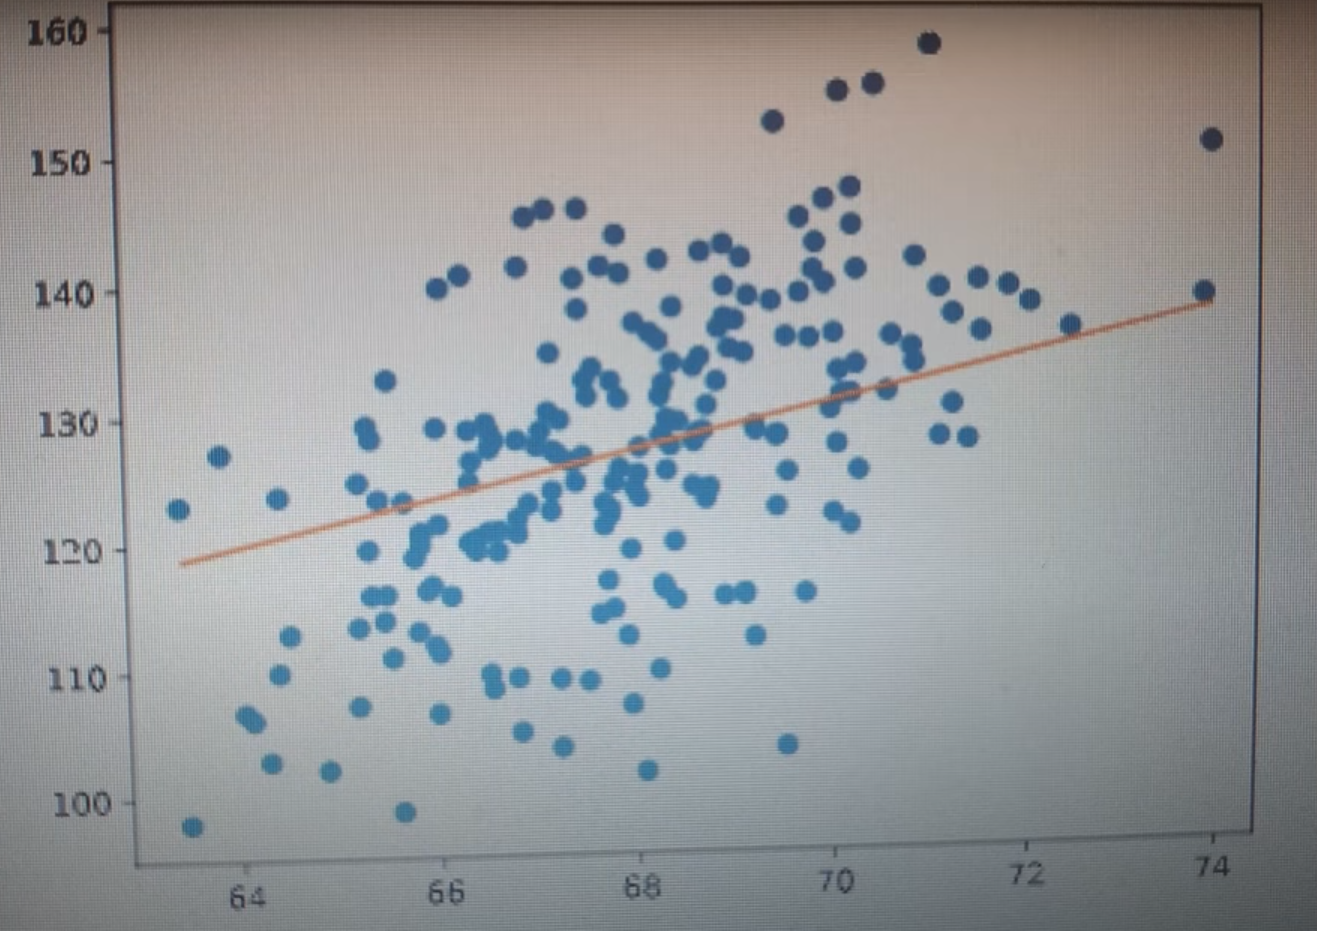
\includegraphics[width=0.04\textwidth]{latex/images/meme.PNG}
    \end{figure}

    \noindent
    Die Ausgleichsgerade wird somit durch die Steigung a = $\SI{3.3 (11)e-15}{\volt\per\ampere}$ und den y-Achsenabschnitt 
    b = $\SI{-3.5 (19)e8}{\volt\per\coulomb}$ beschrieben.\\
    Nach Gleichung \ref{eqn:vmax} berechnet sich das Verhätnis $\frac{\symup{h}}{\symup{e_0}}$ somit zu $\SI{2.1(7)e4}{\electronvolt}$ und die 
    Austrittsarbeit zu $\SI{1.2(6)}{\electronvolt}$
    \noindent

    \subsection{c)}

    \begin{figure}[H]
        \centering
        \includegraphics[width=0.85\textwidth]{build/plots/gelb.pdf}
        \caption{Die Messreihe für die gelbe Spektrallinie mit $\lambda$ = 578nm.}
        \label{img:gelb}
    \end{figure}

    \noindent
    Das Diagramm beschreibt wie sich bei hohen beschleunigenden Spannungen der Photostrom asymptotisch einem Grenzwert annähert, im mittleren 
    Spannungsbereich annähernd linear abfällt und noch nicht vollständig bei der Grenzspannung $U_{\symup{g}}$ versiegt.\\
    Der sich asymptotisch annähernde Photostrom ist dadurch zu erklären, dass nur begrenzt viele Elektronen bei konstanter Licht Intensität 
    durch den Photoeffekt entstehen. Diese werden in alle möglichen Richtungen verstreut.\\
    Um nun alle diese Elektronen einzufangen, auch die die sich  
    von der Anode weg bewegen, wird ein sehr starkes Feld benötigt.\\
    Es werden bei hohen Spannungen auch nur noch vereinzelt
    weitere Elektronen auf die Anode geleitet. Dies führt zu der asymptotischen Annäherung an den Grenzwert.\\
    Somit wird der Grenzwert durch die 
    Intensität des Lichts bestimmt. Um den Grenzwert bereits bei endlichen Spannungen zu erreichen müsste die Anode eine größere Fläche besitzen
    und die Kathode am besten eine kugelförmige Umschließung erreichen.\\
    Der Effekt, dass bei Erreichen der Grenzspannung kein Photostrom mehr zu sehen ist würde dann nicht vorliegen, da die Elektronen in der Kathode 
    bereits eine durch die Fermi-Dirac-Statistik beschriebene Energie aufweisen. Die Elektronen mit zusätzlicher Energie in Richtung der Anode 
    können somit das Gegenfeld noch überwinden und einen Photostrom erzeugen.
    %Da die Kathode und Anode elektrisch verbunden sind, gleichen sich ihre Fermi-Niveaus aus, das bedeutet, dass sich auch die Austrittsarbeit 
    %für Elektronen ausgleichen. Da bei 20 Grad Celsius bereits Material an der Kathode verdampft, werden somit auch Elektronen an der Anode frei 
    %und durch die Gegenspannung zur Kathode beschleunigt.
    %Diese haben im Gegensatz zu den beim Photoeffekt frei werdenden Elektronen nur geringe kinetische Energien und erreichen bereits bei kleinen 
    %Gegenspannungen vollständig die Kathode.
    können somit das Gegenfeld noch überwinden und einen Photostrom erzeugen.\\
    Da die Kathode und Anode elektrisch verbunden sind gleichen sich ihre Fermi-Niveaus aus. 
    Das bedeutet, dass auch die Austrittsarbeit 
    
    HIER FEHLT NOCH INHALT
    
    Da die Photokathode bereits bei 20 Grad Celsius verdampft und somit Elektronen frei werden kann hier bereits bei kleinen Spann

    

